\documentclass{beamer}


\usetheme{Warsaw}
\usecolortheme{crane}


\title{Boolean Algebra}
\subtitle{Mathematical Methods in the Physical Sciences}
\author{Steve Mazza}
\institute[Naval Postgraduate School]
{ 
    Naval Postgraduate School \\
    Monterey, CA \\
    
\includegraphics[height=3cm]{images/NPS_logo.jpg}
}
\date {SE3030, Winter/2014 \\ Quantitative Methods of Systems Engineering}
\subject{Quantitative Methods of Systems Engineering}


\begin{document}

\frame{\titlepage}


\frame{{Introduction}
    \begin{columns}[c]
    \column{.5\textwidth}
    In 1854 George Boole introduced a 2-state algebra designed to solve logic problems.  Today this algebra is at the heart of network and computer science.
    \column{.5\textwidth}
    \begin{center}
    	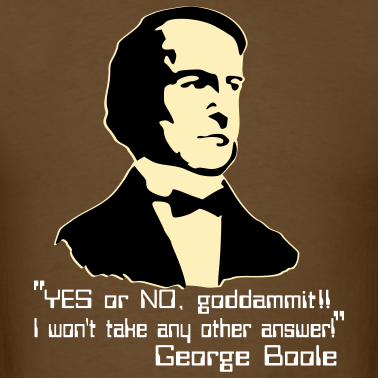
\includegraphics[scale=0.4]{images/boolean-algebra.png}
    \end{center}
    \end{columns}
}


\frame{{Basic Gates}
	\framesubtitle{NOT Gate}
	Receives input $x$ and produces $x'$ where
	\[
	x' = \left\{ 
	\begin{array}{rl}
		1 &\mbox{ if $x=0$} \\
  		0 &\mbox{ if $x=1$}
       	\end{array} \right.
	\]
	The output is the \emph{compliment} of the input.
    	\begin{columns}[c]
    	\column{.5\textwidth}
    	\begin{center}
    	\begin{tabular}{c c}
 		 $x$ & $x'$ \\
 		 \hline
 		 1 & 0 \\
 		 0 & 1 \\
	\end{tabular}
	\end{center}
    	\column{.5\textwidth}
    		\begin{center}
    			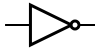
\includegraphics[scale=1]{images/100px-NOT_ANSI.png}
    		\end{center}
    	\end{columns}
}


\frame{{Basic Gates}
	\framesubtitle{AND Gate}
	Receives input $x_1$ and $x_2$ and produces $(x_1\wedge x_2)$ where
	\[
	(x_1\wedge x_2) = \left\{ 
	\begin{array}{rl}
		1 &\mbox{ if $x_1=x_2=1$} \\
  		0 &\mbox{ otherwise}
       	\end{array} \right.
	\]
	There may be more than two inputs but the there is always one output.
    	\begin{columns}[c]
    	\column{.5\textwidth}
    	\begin{center}
    	\begin{tabular}{c c c}
 		 $x_1$ & $x_2$ & $(x_1\wedge x_2)$ \\
 		 \hline
 		 0 & 0 & 0 \\
 		 0 & 1 & 0 \\
 		 1 & 0 & 0 \\
 		 1 & 1 & 1
	\end{tabular}
	\end{center}
    	\column{.5\textwidth}
    		\begin{center}
    			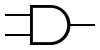
\includegraphics[scale=1]{images/100px-AND_ANSI.png}
    		\end{center}
    	\end{columns}
}


\frame{{Basic Gates}
	\framesubtitle{OR Gate}
	Receives input $x_1$ and $x_2$ and produces $(x_1\vee x_2)$ where
	\[
	(x_1\vee x_2) = \left\{ 
	\begin{array}{rl}
		1 &\mbox{ if $x_1=1$ or $x_2=1$} \\
  		0 &\mbox{ otherwise}
       	\end{array} \right.
	\]
	There may be more than two inputs but the there is always one output.
    	\begin{columns}[c]
    	\column{.5\textwidth}
    	\begin{center}
    	\begin{tabular}{c c c}
 		 $x_1$ & $x_2$ & $(x_1\wedge x_2)$ \\
 		 \hline
 		 0 & 0 & 0 \\
 		 0 & 1 & 1 \\
 		 1 & 0 & 1 \\
 		 1 & 1 & 1
	\end{tabular}
	\end{center}
    	\column{.5\textwidth}
    		\begin{center}
    			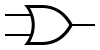
\includegraphics[scale=1]{images/100px-OR_ANSI.png}
    		\end{center}
    	\end{columns}
}


\frame{{Negated and Exclusive Gates}
	\framesubtitle{NOR Gate}
	Receives input $x_1$ and $x_2$ and produces $(x_1\vee x_2)'$ where
	\[
	(x_1\vee x_2)' = \left\{ 
	\begin{array}{rl}
		1 &\mbox{ if $x_1=x_2=0$} \\
  		0 &\mbox{ otherwise}
       	\end{array} \right.
	\]
	There may be more than two inputs but the there is always one output.
    	\begin{columns}[c]
    	\column{.5\textwidth}
    	\begin{center}
    	\begin{tabular}{c c c}
 		 $x_1$ & $x_2$ & $(x_1\wedge x_2)'$ \\
 		 \hline
 		 0 & 0 & 1 \\
 		 0 & 1 & 0 \\
 		 1 & 0 & 0 \\
 		 1 & 1 & 0
	\end{tabular}
	\end{center}
    	\column{.5\textwidth}
    		\begin{center}
    			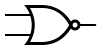
\includegraphics[scale=1]{images/100px-NOR_ANSI.png}
    		\end{center}
    	\end{columns}
}


\frame{{Negated and Exclusive Gates}
	\framesubtitle{NAND Gate}
	Receives input $x_1$ and $x_2$ and produces $(x_1\wedge x_2)'$ where
	\[
	(x_1\wedge x_2)' = \left\{ 
	\begin{array}{rl}
		1 &\mbox{ if $x_1=0$ or $x_2=0$} \\
  		0 &\mbox{ otherwise}
       	\end{array} \right.
	\]
	There may be more than two inputs but the there is always one output.
    	\begin{columns}[c]
    	\column{.5\textwidth}
    	\begin{center}
    	\begin{tabular}{c c c}
 		 $x_1$ & $x_2$ & $(x_1\wedge x_2)'$ \\
 		 \hline
 		 0 & 0 & 1 \\
 		 0 & 1 & 1 \\
 		 1 & 0 & 1 \\
 		 1 & 1 & 0
	\end{tabular}
	\end{center}
    	\column{.5\textwidth}
    		\begin{center}
    			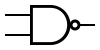
\includegraphics[scale=1]{images/100px-NAND_ANSI.png}
    		\end{center}
    	\end{columns}
}


\frame{{Negated and Exclusive Gates}
	\framesubtitle{XOR Gate}
	Receives input $x_1$ and $x_2$ and produces $(x_1\oplus x_2)$ where
	\[
	(x_1\oplus x_2) = \left\{ 
	\begin{array}{rl}
		1 &\mbox{ if only $x_1=0$ or only $x_2=1$} \\
  		0 &\mbox{ otherwise}
       	\end{array} \right.
	\]
	There may be more than two inputs but the there is always one output.
	The XNOR gate implements the logical expressions: $x_1 \wedge \overline{x_2} \vee \overline{x_1} \wedge x_2$ and $(x_1 \vee x_2) \wedge \overline{x_1 \wedge x_2}$.
    	\begin{columns}[c]
    	\column{.5\textwidth}
    	\begin{center}
    	\begin{tabular}{c c c}
 		 $x_1$ & $x_2$ & $(x_1\oplus x_2)$ \\
 		 \hline
 		 0 & 0 & 0 \\
 		 0 & 1 & 1 \\
 		 1 & 0 & 1 \\
 		 1 & 1 & 0
	\end{tabular}
	\end{center}
    	\column{.5\textwidth}
    		\begin{center}
    			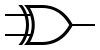
\includegraphics[scale=1]{images/100px-XOR_ANSI.png}
    		\end{center}
    	\end{columns}
}


\frame{{Negated and Exclusive Gates}
	\framesubtitle{XNOR Gate}
	Receives input $x_1$ and $x_2$ and produces $(x_1\oplus x_2)'$ where
	\[
	(x_1\oplus x_2)' = \left\{ 
	\begin{array}{rl}
		1 &\mbox{ if $x_1=x_2$} \\
  		0 &\mbox{ otherwise}
       	\end{array} \right.
	\]
	There may be more than two inputs but the there is always one output. 
	The XNOR gate implements the logical expression: $x_1 \wedge x_2 \vee \overline{x_1} \wedge \overline{x_2}$.
    	\begin{columns}[c]
    	\column{.5\textwidth}
    	\begin{center}
    	\begin{tabular}{c c c}
 		 $x_1$ & $x_2$ & $(x_1\oplus x_2)'$ \\
 		 \hline
 		 0 & 0 & 1 \\
 		 0 & 1 & 0 \\
 		 1 & 0 & 0 \\
 		 1 & 1 & 1
	\end{tabular}
	\end{center}
    	\column{.5\textwidth}
    		\begin{center}
    			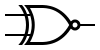
\includegraphics[scale=1]{images/100px-XNOR_ANSI.png}
    		\end{center}
    	\end{columns}
}


\frame{{Combinatorial Circuit}
  In digital circtuis, low voltages represent 0 and high voltages represent 1.
	\begin{block}{Combinatorial Circuit}
    A combinatorial circuit iis a circuit which produces a unique output for every combination of inputs.
	\end{block}
  Negative feedback from an op-amp provides a counter-example since the feedback loop negates the uniqueness of the output for every combination of inputs.
}


\frame{{Boolean Expression}
	\begin{block}{Boolean Expression}
    A boolean expression is any expression built up from individual state variables (e.g., $x_1, x_2$) by applyting the operations $\wedge, \vee$, and $'$ a finite number of times.
	\end{block}
  The output of a combinatorial circuit is a boolean expression.
}


\frame{{Boolean Expression}
  \framesubtitle{Properties}
  \begin{itemize}
    \item Associative Laws: $\forall a,b,c \in {0,1}$
      \begin{itemize}
        \item $(a\wedge b)\wedge c=a\wedge(b\wedge c)$
        \item $(a\vee b)\vee c=a\vee(b\vee c)$
      \end{itemize}
    \item Identity Laws: $\forall a \in {0,1}$
      \begin{itemize}
        \item $(a\wedge 1)=a$
        \item $(a\vee 0)=a$
      \end{itemize}
    \item Commutative Laws: $\forall a,b \in {0,1}$
      \begin{itemize}
        \item $(a\wedge b)=(b\wedge a)$
        \item $(a\vee b)=(b\vee a)$
      \end{itemize}
    \item Complement Laws: $\forall z \in {0,1}$
      \begin{itemize}
        \item $(a\wedge a')=0$
        \item $(a\vee a')=1$
      \end{itemize}
    \item Distributive Laws: $\forall a,b,c \in {0,1}$
      \begin{itemize}
        \item $a\wedge(b\vee c)=(a\wedge b)\vee(a\wedge c)$
        \item $a\vee(b\wedge c)=(a\vee b)\wedge(a\vee c)$
      \end{itemize}
  \end{itemize}
}


\frame{{Boolean Expression}
  \framesubtitle{deMorgan's Laws}
  \begin{align*}
    (x_1\wedge x_2)' &= x_1'\vee x_2' \\
    (x_1\vee x_2)' &= x_1'\wedge x_2'
  \end{align*}
  We demonstrate the first example.
  \begin{center}
    \begin{tabular}{cccccc}
      $x_1$ & $x_2$ & $(x_1\wedge x_2)'$ & $x_1'$ & $x_2'$ & $x_1'\vee x_2'$ \\
      \hline
      1 & 1 & 0 & 0 & 0 & 0 \\
      1 & 0 & 1 & 0 & 1 & 1 \\
      0 & 1 & 1 & 1 & 0 & 1 \\
      0 & 0 & 1 & 1 & 1 & 1
    \end{tabular}
  \end{center}
}


\frame{{Equivalent Combinatorial Circuits}
  Two combinatorial circuits are said to be equivalent if they produce the same output for the same input.

  \begin{exampleblock}{Example}
    \begin{align}
    (x_1\wedge x_2)' &= y \\
    (x_1'\vee x_2') &= y
    \end{align}
  \end{exampleblock}
  \begin{columns}[c]
    \column{.5\textwidth}
    \begin{center}
    \begin{table}
    \begin{tabular}{ccc}
     $x_1$ & $x_2$ & $y$ \\
     \hline
     1 & 1 & 0 \\
     1 & 0 & 1 \\
     0 & 1 & 1 \\
     0 & 0 & 1
    \end{tabular}
    \caption{(example 1)}
    \end{table}
    \end{center}
    \column{.5\textwidth}
    \begin{center}
    \begin{table}
    \begin{tabular}{ccc}
     $x_1$ & $x_2$ & $y$ \\
     \hline
     1 & 1 & 0 \\
     1 & 0 & 1 \\
     0 & 1 & 1 \\
     0 & 0 & 1
    \end{tabular}
    \caption{(example 2)}
    \end{table}
    \end{center}
  \end{columns}
}


\frame{{Boolean Algebra}
  A Boolean algebra $B$ consists of a set $S$ together with any two binary operations $\wedge$ and $\vee$, a singular operation $'$ and two specific elements 0 and 1 on $S$ such that the following laws hold.
  \begin{itemize}
    \item Associative Laws: $\forall a,b,c \in S$
      \begin{itemize}
        \item $(a\wedge b)\wedge c=a\wedge(b\wedge c)$
        \item $(a\vee b)\vee c=a\vee(b\vee c)$
      \end{itemize}
    \item Identity Laws: $\forall a \in S$
      \begin{itemize}
        \item $(a\wedge 1)=a$
        \item $(a\vee 0)=a$
      \end{itemize}
    \item Commutative Laws: $\forall a,b \in S$
      \begin{itemize}
        \item $(a\wedge b)=(b\wedge a)$
        \item $(a\vee b)=(b\vee a)$
      \end{itemize}
    \item Complement Laws: $\forall z \in S$
      \begin{itemize}
        \item $(a\wedge a')=0$
        \item $(a\vee a')=1$
      \end{itemize}
    \item Distributive Laws: $\forall a,b,c \in S$
      \begin{itemize}
        \item $a\wedge(b\vee c)=(a\wedge b)\vee(a\wedge c)$
        \item $a\vee(b\wedge c)=(a\vee b)\wedge(a\vee c)$
      \end{itemize}
   \end{itemize}
}


\frame{{Dual of a Statement}
	Two Boolean expressions are said to be the dual of each other if one expression is obtained from the other by the following replacements:
  \begin{itemize}
    \item replace 0 by 1
    \item replace 1 by 0
    \item replace $\wedge$ by $\vee$
    \item replace $\vee$ by $\wedge$
  \end{itemize}
  \begin{exampleblock}{Example 1}
    $(x\wedge y)' = x'\vee y'$ is the dual of $(x\vee y)' = x'\wedge y'$
  \end{exampleblock}
  \begin{exampleblock}{Example 2}
    $(x\wedge 1)=x$ is the dual of $(x\vee 0)=x$
  \end{exampleblock}
}


\frame{{Boolean Function}
  Let $B=(S, \vee, \wedge, ', 0, 1)$ be a Boolean algebra and let $X(x_1, x_2, x_3, \dots, x_n)$ be a Boolean expression in $n$ variables.  A function $f:B^n\rightarrow B$ is called a Boolean function if $f$ is of the form
  \[ f(x_1, x_2, x_3, \dots, x_n) = X(x_1, x_2, x_3, \dots, x_n) \]
}


\frame{{Various Normal Forms}
	\begin{itemize}
    \item Disjunctive normal form: a Boolean function $f:B^n\rightarrow B$ consisting of a sum of elemantary products.
    \item Conjunctive normal form: a Boolean function $f:B^n\rightarrow B$ consisting of a product of elemantary sums.
	\end{itemize}
}


\frame{{Questions?}
	\begin{center}
		
\includegraphics[width=.7\textwidth]{images/fin.png}
	\end{center}
}

\end{document}
